\documentclass[12pt,a4paper]{article}
\usepackage[a4paper,margin=2cm]{geometry}
\usepackage{fontspec}
\setmainfont{Times New Roman}
\usepackage{polyglossia}
\setdefaultlanguage{russian}
\setotherlanguage{english}
\usepackage{amsmath}
\usepackage{unicode-math}
\setmathfont{STIX Two Math}
\usepackage{graphicx,booktabs,tabularx,array,caption,setspace,indentfirst}
\usepackage[hidelinks]{hyperref}
\captionsetup{labelformat=empty,font=small,justification=centering}
\setlength{\parindent}{1.25cm}
\onehalfspacing
\renewcommand{\arraystretch}{1.15}
\newcolumntype{Y}{>{\raggedright\arraybackslash}X}
\begin{document}
\begin{singlespace}\small
\noindent Научная статья\\
\noindent УДК 004.912:004.89
\begin{center}\large\textbf{ЛОКАЛЬНЫЙ КОНТУР RAG С НЕЗАВИСИМОЙ NLI-ВЕРИФИКАЦИЕЙ УТВЕРЖДЕНИЙ ДЛЯ ПОИСКА ОТВЕТОВ ПО ТЕХНИЧЕСКОЙ ДОКУМЕНТАЦИИ}\\[6pt]
\normalsize\textbf{Егор Дмитриевич Мясников}\\
\small Российский университет дружбы народов имени Патриса Лумумбы, Москва, Россия\\Hloykanika@gmail.com\end{center}
\textbf{Аннотация.} \textbf{Введение.} Большие языковые модели при работе с нормативной и технической документацией порождают правдоподобные, но не подтверждённые источником утверждения, искажающие числовые допуски и модальность требований, а режим коммерческой тайны исключает облачные сервисы. Цель исследования состоит в построении и экспериментальной оценке локального многорубежного контура генерации с дополнением извлечением, в котором каждое утверждение ответа проходит независимую проверку, а неподтверждённые утверждения не публикуются. \textbf{Методы.} Контур FactRAG-NLI объединяет двухэтапный гибридный поиск (BM25 и BGE-M3 с объединением Reciprocal Rank Fusion и переранжированием bge-reranker-v2-m3), генерацию ответа моделью Qwen3.8-27B со ссылками на источники и двухмодельный верификатор: логистического судью по признакам классификаторов mDeBERTa-v3 и BGE-M3-zeroshot с детерминированным контролем числовых и буквенно-цифровых якорей. Полноту ответа восстанавливают повторный проход с рассуждением после частичного удаления утверждений и условный перевод вопроса на язык источников после отказа. Оценка выполнена на 1307 вопросах (технический набор v3 и XQuAD) с замороженным разбиением на выборки dev и test, контролем детерминизма по SHA-256 и точным тестом Мак-Немара. \textbf{Результаты.} Доля верных ответов выросла с 90,2 до 91,3 \% (+18/−4 вопроса, p = 0,004), на техническом наборе с 86,4 до 90,9 \%. Доля галлюцинаций на 269 неотвечаемых и провокационных вопросах составила 0,7 \%, доля ложных отказов 6,7 \%. Повтор залогированных черновиков воспроизводит 1307 исходов из 1307. Медианное время полного ответа на RTX 3090 составило от 4,4 до 6,1 с. \textbf{Заключение.} Независимая многорубежная проверка смещает ошибки в сторону отказа при малых вычислительных затратах. Остаточные ошибки связаны с ограничениями NLI на модальностях, таблицах и межъязыковых формулировках и с качеством эталонной разметки.

\textbf{Ключевые слова:} генерация с дополнением извлечением (RAG), логический вывод на естественном языке (NLI), верификация утверждений, гибридный поиск, переранжирование, межъязыковой поиск, большие языковые модели, техническая документация

\textbf{Для цитирования:} Мясников Е. Д. Локальный контур RAG с независимой NLI-верификацией утверждений для поиска ответов по технической документации // Вестник Российского университета дружбы народов. Серия: Инженерные исследования. 2026. Т. XX, № X. С. XX–XX.

\begin{otherlanguage}{english}
\noindent Original article
\begin{center}\large\textbf{A Local RAG Pipeline with Independent NLI-Based Claim Verification for Question Answering over Technical Documentation}\\[6pt]
\normalsize\textbf{Egor D. Myasnikov}\\
\small Peoples' Friendship University of Russia named after Patrice Lumumba, Moscow, Russia\\Hloykanika@gmail.com\end{center}
\textbf{Abstract.} \textbf{Introduction.} Large language models applied to normative and technical documentation produce plausible but unsupported claims that distort numerical tolerances and requirement modality, while trade-secret constraints rule out cloud services. The aim of the study is to build and evaluate a local multi-stage retrieval-augmented generation pipeline in which every claim of an answer is verified independently and unsupported claims are never published. \textbf{Methods.} The FactRAG-NLI pipeline combines two-stage hybrid retrieval (BM25 and BGE-M3 fused by Reciprocal Rank Fusion and reranked by bge-reranker-v2-m3), cited answer generation by Qwen3.8-27B, and a two-model verifier: a logistic judge over the features of the mDeBERTa-v3 and BGE-M3-zeroshot classifiers with deterministic checks of numerical and alphanumeric anchors. Answer completeness is restored by a reasoning pass after a partially trimmed draft and by a conditional translation of the question into the language of the sources after a refusal. The evaluation covers 1307 questions (the technical set v3 and XQuAD) with a frozen dev/test split, SHA-256 determinism control and the exact McNemar test. \textbf{Results.} Accuracy increased from 90.2\% to 91.3\% (+18/−4 questions, p = 0.004) and from 86.4\% to 90.9\% on the technical set. The hallucination rate on 269 unanswerable and adversarial questions is 0.7\% and the false refusal rate is 6.7\%. Replaying the logged drafts reproduces 1307 of 1307 outcomes. The median end-to-end latency on an RTX 3090 is 4.4 to 6.1 s. \textbf{Conclusion.} Independent multi-stage verification shifts errors towards refusal at a low computational cost. The remaining errors stem from NLI limitations on modality, tables and cross-lingual wording and from the quality of the reference labels.

\textbf{Keywords:} retrieval-augmented generation (RAG), natural language inference (NLI), claim verification, hybrid retrieval, reranking, cross-lingual retrieval, large language models, technical documentation

\textbf{For citation:} Myasnikov E. D. A Local RAG Pipeline with Independent NLI-Based Claim Verification for Question Answering over Technical Documentation. RUDN Journal of Engineering Research. 2026;XX(X):XX–XX. (In Russ.)
\end{otherlanguage}
\end{singlespace}

\section*{Введение}
Большие языковые модели демонстрируют высокую беглость генерации, однако склонность к галлюцинациям, то есть к порождению правдоподобных, но не подтверждённых источником утверждений, систематически фиксируется в обзорных исследованиях [1; 2]. Для нормативной и технической документации такие ошибки критичны по двум причинам. Во-первых, значимую часть содержания составляют числовые допуски, пороговые значения, коды и идентификаторы, искажение которых меняет инженерное решение. Во-вторых, требования выражаются модальными глаголами MUST, SHOULD и MAY, семантика которых нормативно закреплена [3]: подмена обязательного требования рекомендательным сохраняет тематическую близость ответа, но меняет его юридическое и техническое содержание.

Генерация с дополнением извлечением (Retrieval-Augmented Generation, RAG) [4; 5] снижает зависимость ответа от параметрической памяти модели, но не гарантирует, что каждое утверждение следует из процитированного фрагмента. Генератор способен объединить несколько источников в неверный вывод, перенести условие из соседнего раздела или сохранить ссылку при искажённом содержании [6]. Наличие ссылки поэтому не является достаточным признаком достоверности. Дополнительное ограничение связано с конфиденциальностью: проектная и эксплуатационная документация предприятия, как правило, составляет коммерческую тайну [7], и все вычисления (индексация, поиск, генерация и проверка) должны выполняться в изолированном локальном контуре.

Существующие подходы решают задачу контроля достоверности частично. Модели с самокритикой [8] встраивают проверку в сам генератор, что лишает её независимости. Методы оценки фактической точности на основе декомпозиции на атомарные утверждения [9], автоматизированной оценки RAG-конвейеров [10] и проверки согласованности средствами логического вывода на естественном языке (Natural Language Inference, NLI) [11; 12] разработаны преимущественно как инструменты офлайн-оценки, а не как механизм допуска ответа в режиме реального времени. Одиночный NLI-классификатор, применённый как фильтр, к тому же неустойчив к перефразированию, модальным конструкциям и смешению языков, а вероятностная оценка не распознаёт подмену числа или идентификатора при высоком лексическом перекрытии.

В предыдущей версии работы был описан ранний прототип контура FactRAG-NLI: модель Qwen2.5-14B-Instruct, переранжировщик BGE-Reranker-Large и одиночный классификатор mDeBERTa-v3 на мобильной видеокарте с 8 ГБ памяти, оценка на 50 сценариях. В качестве направлений развития там были названы расширение корпуса, калибровка порогов на независимой выборке, абляционный анализ и дополнение вероятностной проверки детерминированным контролем числовых и модальных отношений. Настоящая статья описывает итоговое состояние контура, в котором все эти направления реализованы и проверены на 1307 вопросах.

Научная новизна работы состоит в сочетании четырёх механизмов в едином детерминированном контуре допуска ответа: двухэтапного гибридного поиска с весом разреженного канала, зависящим от покрытия запроса словарём индекса; двухмодельного верификатора, в котором калиброванный логистический судья объединяет оценки классификаторов mDeBERTa-v3 и BGE-M3-zeroshot, а детерминированный контроль числовых и буквенно-цифровых якорей действует как жёсткое правило; повторного прохода с рассуждением после частичного удаления утверждений (llm\_think\_on\_trim), результат которого принимается только при полной проверке; условного межъязыкового перевода вопроса после отказа (G3, QUERY\_TRANSLATION). Каждый механизм вводился как отдельная гипотеза с заранее заданными критериями принятия и подтверждался попарным сравнением по вопросам.

Цель исследования состоит в построении и экспериментальной оценке локального многорубежного контура FactRAG-NLI для поиска ответов по технической документации, в котором каждое утверждение ответа проходит независимую проверку. Для достижения цели решены следующие задачи:

-- разработка инкрементальной индексации со структурным разбором заголовков и таблиц;\par
-- построение двухэтапного гибридного поиска с переранжированием и гейтом релевантности;\par
-- формализация двухмодельной верификации утверждений с детерминированным контролем якорей;\par
-- разработка адаптивных механизмов восстановления полноты ответа и преодоления ложных отказов;\par
-- построение воспроизводимой методики оценки с замороженным разбиением dev/test и попарными статистическими тестами и экспериментальная оценка контура.\par
\section*{Методы}
\subsection*{\textit{Архитектура контура}}
Архитектура FactRAG-NLI включает пять функциональных уровней (рисунок 1). Уровень конфигурации и ресурсов задаёт типизированные параметры (settings.py) и профиль развёртывания. Документный уровень выполняет разбор, дедупликацию и сегментацию. Уровень поиска, генерации и проверки реализует гибридное извлечение, переранжирование, генерацию и верификацию. Уровень оркестрации (pipeline.py) сериализует доступ к видеокарте и встроенному индексу Qdrant, управляет адаптивными проходами и формирует типизированный результат. Уровень интерфейсов и оценки предоставляет программный интерфейс HTTP, веб-интерфейс и средства корпусной оценки (evaluate\_suite.py).

\begin{figure}[htbp]\centering
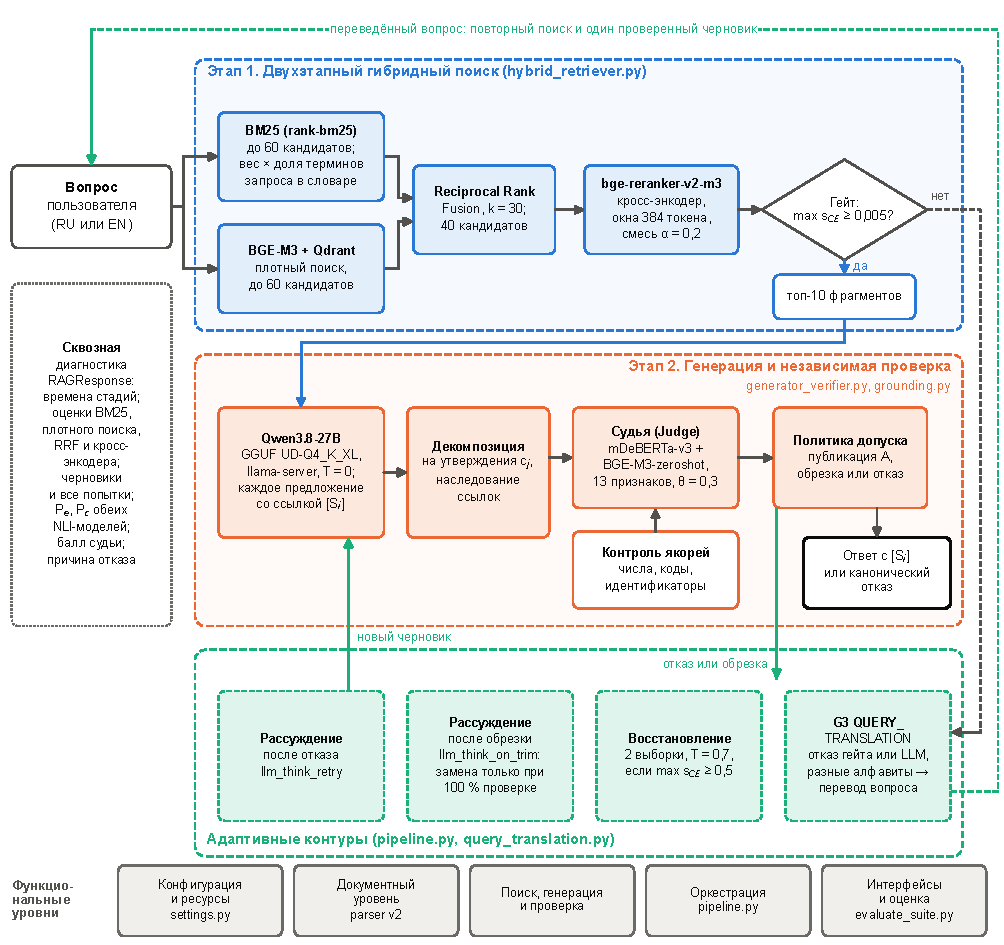
\includegraphics[width=\textwidth]{figures/fig1.pdf}
\caption{Рисунок 1 – Архитектура контура FactRAG-NLI: маршрут запроса, адаптивные контуры и функциональные уровни}
\end{figure}

Ключевое архитектурное решение состоит в том, что черновой ответ генератора не публикуется до прохождения политики допуска: пользователю передаётся либо множество подтверждённых утверждений со ссылками, либо канонический отказ. Отказ возможен на двух рубежах: до генерации, если ни один фрагмент не преодолел порог релевантности, и после генерации, если подтверждение утверждений недостаточно. Адаптивные контуры запускаются только по формальным условиям и никогда не публикуют непроверенный текст.

\subsection*{\textit{Инкрементальная индексация и структурный разбор}}
Конвейер индексации (рисунок 2) принимает документы форматов PDF с текстовым слоем, DOCX, TXT и Markdown. До разбора создаётся снимок файла и вычисляется хеш SHA-256, который служит идентификатором документа: повторно загруженный файл, в том числе под другим именем, пропускается без пересчёта векторов, а изменённое содержимое регистрируется как новая версия. Каждый фрагмент хранит хеш документа, порядковый номер и ожидаемое число фрагментов; документ, индексация которого прервана, исключается из поиска до повторной загрузки.

\begin{figure}[htbp]\centering
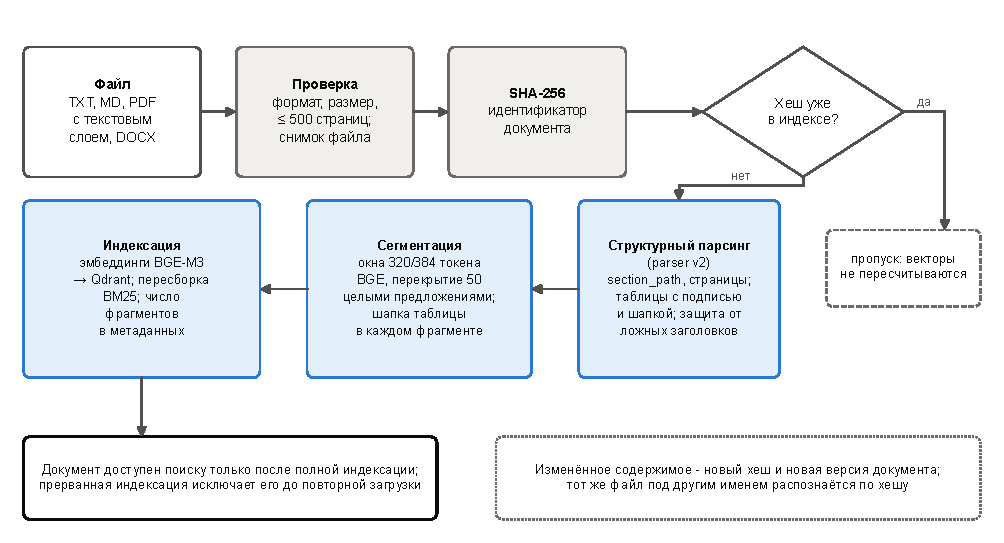
\includegraphics[width=\textwidth]{figures/fig2.pdf}
\caption{Рисунок 2 – Конвейер инкрементальной индексации и контроля целостности документов}
\end{figure}

Структурный разбор сохраняет путь раздела section\_path, номера страниц и таблицы. Анализ ошибок показал, что исходный разбор англоязычных документов создавал ложные разделы: заголовком считалась любая строка, начинающаяся с числа, и под такими разделами оказывались 38 \% фрагментов технического корпуса; таблицы делились по строкам без шапки, а подписи вида «Table N:» не распознавались. Итоговая версия разбора (parser v2) отличает заголовок от пункта списка, адреса и строки оглавления по набору формальных признаков, распознаёт подписи таблиц, преобразует таблицы в разметке RFC в формат Markdown, объединяет многоуровневые шапки и повторяет подпись и шапку таблицы в каждом её фрагменте. Для русскоязычных документов результат разбора совпадает с исходным побайтно.

Сегментация оценочного индекса выполняется окнами с целевым размером 320 и максимальным размером 384 токена токенизатора BGE с перекрытием 50 токенов; перекрытие формируется только целыми предложениями, и фрагмент не пересекает границу раздела. Для документов, загружаемых пользователем через программный интерфейс, применяется профиль 650/800 токенов с перекрытием 75. Меньший профиль оценочного индекса выбран так, чтобы пара «фрагмент – утверждение» укладывалась в 512 токенов входа NLI-классификатора без усечения.

\subsection*{\textit{Двухэтапный гибридный поиск}}
На первом этапе запрос обрабатывается двумя независимыми методами: разреженным поиском BM25 [13], чувствительным к точным совпадениям терминов, номеров разделов и кодов, и плотными векторными представлениями BGE-M3 [14] во встроенном индексе Qdrant [15], отражающими семантическое, в том числе межъязыковое, сходство. Каждый метод извлекает до 60 кандидатов. Ранжированные списки объединяются формулой Reciprocal Rank Fusion [16]:

\begin{equation}
s_{\mathrm{RRF}}(d) = \sum_{m \in \{\mathrm{BM25},\, \mathrm{BGE}\}} \frac{w_m}{k + \mathrm{rank}_m(d)}, \quad k = 30
\tag{1}
\end{equation}
\noindent где $\mathrm{rank}_m(d)$ – позиция фрагмента $d$ в списке метода $m$; $w_m$ – вес метода; $k$ – параметр сглаживания.

Для русскоязычного вопроса к англоязычному документу BM25 может совпасть только по латинским идентификаторам, и несовпавшие слова не должны размывать объединение. Поэтому вес разреженного канала масштабируется долей терминов запроса, присутствующих в словаре индекса:

\begin{equation}
w_{\mathrm{BM25}} = w_0 \cdot \frac{|T(q) \cap V|}{|T(q)|}
\tag{2}
\end{equation}
\noindent где $T(q)$ – множество терминов запроса $q$; $V$ – словарь разреженного индекса; $w_0 = 1$ – базовый вес; вес плотного канала $w_{\mathrm{BGE}} = 1$.

На второй этап передаются 40 лучших кандидатов объединённого списка. Кросс-энкодер bge-reranker-v2-m3 [17; 18; 19] оценивает пару «вопрос – фрагмент» совместным кодированием; длинные фрагменты оцениваются перекрывающимися окнами по 384 токена с максимумом по окнам. Итоговое упорядочение использует нормированную смесь:

\begin{equation}
s(d) = \alpha \, \frac{s_{\mathrm{RRF}}(d)}{s_{\max}} + (1 - \alpha)\, s_{\mathrm{CE}}(d), \quad s_{\max} = \frac{w_{\mathrm{BM25}} + w_{\mathrm{BGE}}}{k + 1}
\tag{3}
\end{equation}
\noindent где $s_{\mathrm{CE}}(d) \in (0, 1)$ – оценка кросс-энкодера после сигмоиды; $\alpha = 0{,}2$ – вес объединённого ранга; $s_{\max}$ – максимально достижимая оценка RRF.

Гейт релевантности действует как первый рубеж отказа:

\begin{equation}
\mathrm{gate}(q) = \left[\max_{d \in D_{40} \setminus H} s_{\mathrm{CE}}(d) \ge \tau\right], \quad \tau = 0{,}005
\tag{4}
\end{equation}
\noindent где $D_{40}$ – кандидаты второго этапа; $H$ – фрагменты, состоящие только из заголовка. Если гейт открыт, генератору передаются десять фрагментов с наибольшей оценкой (3); иначе формируется канонический отказ relevance\_threshold\_not\_met без обращения к генератору. Порог $\tau$ откалиброван под шкалу bge-reranker-v2-m3: для прежнего переранжировщика BGE-Reranker-Large использовалось значение 0,05.

Качество поиска оценивается метриками Recall@5 и MRR@10 по отвечаемым вопросам:

\begin{equation}
\mathrm{Recall@}K = \frac{1}{|Q|} \sum_{q \in Q} \frac{|G_q \cap R_q^{K}|}{|G_q|}, \qquad \mathrm{MRR@}K = \frac{1}{|Q|} \sum_{q \in Q} \frac{\mathbf{1}[r_q \le K]}{r_q}
\tag{5}
\end{equation}
\noindent где $Q$ – множество вопросов; $G_q$ – эталонные фрагменты вопроса $q$; $R_q^{K}$ – первые $K$ фрагментов выдачи; $r_q$ – позиция первого эталонного фрагмента.

\subsection*{\textit{Локальный инференс генератора}}
Генератором служит модель Qwen3.8-27B семейства Qwen3 [20; 21], квантованная в формат GGUF профиля UD-Q4\_K\_XL [22] и обслуживаемая сервером llama-server [23] через совместимый программный интерфейс HTTP, ограниченный адресом обратной петли. На видеокарте с 24 ГБ памяти модель размещается целиком: на устройство выгружаются все слои, окно контекста составляет 8192 токена, используется механизм flash attention. Профиль qwen38-27b-hybrid генерирует черновик без рассуждения при температуре 0 и фиксированном зерне 42 с ограничением 512 токенов; проход с рассуждением (бюджет рассуждения 640 токенов, до 1024 токенов ответа) запускается только адаптивными механизмами, описанными ниже. Генератор получает инструкцию сопровождать каждое предложение ссылкой вида [S$_i$] и при отсутствии сведений дословно воспроизводить канонический отказ; ответ на ложную предпосылку вопроса должен начинаться с явного опровержения.

Эмбеддинги запросов BGE-M3 вычисляются на центральном процессоре в обоих режимах верификатора. Это решение принято после того, как анализ ранней конфигурации показал методическую ошибку сравнения: при вычислении эмбеддингов на разных устройствах плотный поиск расходился в последних знаках, и 233 из 1148 сравнимых вопросов получали разный порядок контекста, а значит и разные черновики. После выравнивания режимы различаются только верификатором; перенос эмбеддингов на процессор освобождает около 1,1 ГБ видеопамяти ценой примерно 60 мс на запрос. Сводные параметры проверенного профиля представлены в таблице 1.

\begin{table}[htbp]
\begin{singlespace}\footnotesize
\noindent Таблица 1 – Параметры проверенного профиля конвейера (профиль qwen38-27b-hybrid, верификатор judge)\\[2pt]
\begin{tabularx}{\textwidth}{YYY}
\toprule
\textbf{Стадия} & \textbf{Модель или метод} & \textbf{Ключевые параметры} \\
\midrule
Разбор и сегментация & parser v2, токенизатор BGE & фрагменты 320/384 токена, перекрытие 50; подпись и шапка таблицы в каждом фрагменте \\
Разреженный поиск & BM25 (rank-bm25) & до 60 кандидатов; вес по формуле (2) \\
Плотный поиск & BGE-M3, Qdrant & до 60 кандидатов; эмбеддинги запросов на CPU \\
Объединение & Reciprocal Rank Fusion & $k = 30$; 40 кандидатов на переранжирование \\
Переранжирование & bge-reranker-v2-m3 & окна 384 токена; $\alpha = 0{,}2$; гейт $\tau = 0{,}005$ по лучшему фрагменту; топ-10 \\
Генерация & Qwen3.8-27B, GGUF UD-Q4\_K\_XL & llama-server, все слои на GPU, контекст 8192, T = 0, зерно 42, до 512 токенов \\
Рассуждение & тот же генератор & бюджет 640 токенов, ответ до 1024 токенов; после отказа и после обрезки \\
Восстановление & тот же генератор & 2 выборки при T = 0,7, если $\max s_{\mathrm{CE}} \ge 0{,}5$ \\
Перевод вопроса (G3) & тот же генератор & после отказа гейта или LLM при различии алфавитов \\
Верификация & mDeBERTa-v3-base, BGE-M3-zeroshot, судья & 13 признаков; $\theta = 0{,}3$; вето 0,9; входы 512 и 1024 токена \\
Контроль якорей & grounding.py & числа, литералы и идентификаторы в тексте и заголовках источника \\
\bottomrule
\end{tabularx}
\end{singlespace}
\end{table}

\subsection*{\textit{Независимая верификация утверждений}}
Верификация отделена от генерации и выполняется моделями, не имеющими доступа к рассуждениям генератора. Черновой ответ декомпозируется на утверждения $C = \{c_1, \ldots, c_m\}$ на уровне предложений: сегментатор сохраняет десятичные числа, номера разделов и сокращения, а утверждение без собственной ссылки наследует ссылку предыдущего предложения. Для каждого утверждения $c_j$ определяется множество процитированных источников $\mathrm{Src}(c_j)$; утверждение без ссылки получает статус UNVERIFIED. Высказывания об отсутствии сведений в источниках и вердикты вида «нет» не проверяются как факты и не учитываются как снятые.

Верификатор прошёл три стадии развития. В раннем прототипе одиночный классификатор mDeBERTa-v3 [24; 25] сравнивал утверждение со всем фрагментом по порогам $P(\mathrm{entailment}) > 0{,}40$ и $P(\mathrm{contradiction}) < 0{,}20$. Анализ ошибок показал, что длинный фрагмент смешивает подтверждающее предложение с соседними строками, кодами и условиями, и классификатор сообщает противоречие для утверждения, которое фрагмент содержит дословно. Во второй версии (верификатор v2, режим rules) посылка очищается от разметки, к ней добавляются окна из одного-двух предложений и варианты с заголовком «Документ. Раздел.», а поддержку дают окно с высокими порогами (0,8 и 0,05), окно со всеми якорями утверждения при пониженных порогах (0,4 и 0,2) или дословное совпадение кодового фрагмента длиной от 12 символов.

Итоговая версия (режим judge) добавляет вторую модель: классификатор BGE-M3-zeroshot [26], дообученный для задачи NLI на основе BGE-M3. Обе модели оценивают одни и те же посылки (фрагмент, окна и варианты с заголовком), и для каждого процитированного источника $S_i$ формируется вектор из 13 признаков $\varphi(c_j, S_i)$: логиты максимальной вероятности следования каждой модели и их среднего, максимальные вероятности противоречия, оценки по целому фрагменту, лексическое перекрытие, признак дословного кодового фрагмента, признаки наличия якорей и их присутствия в источнике. Вероятность поддержки вычисляет логистический судья:

\begin{equation}
p(c_j, S_i) = \sigma\left(\beta_0 + \symbf{\beta}^{\mathsf{T}} \varphi(c_j, S_i)\right), \quad \sigma(z) = \frac{1}{1 + e^{-z}}
\tag{6}
\end{equation}
\noindent где $\beta_0$ и $\symbf{\beta}$ – коэффициенты, подобранные на стресс-наборе утверждений половины dev ранее выполненного прогона; $\sigma$ – логистическая функция. Стресс-набор содержит верные утверждения черновиков и их детерминированные искажения: подмену ответа другим ответом того же типа, подмену числа, вставку отрицания и перенос утверждения из другого документа.

Детерминированный контроль якорей действует как жёсткое правило. Множество якорей $A(c_j)$ включает числа (в том числе с разделителями разрядов и десятичными знаками), шестнадцатеричные и двоичные литералы, ключи командной строки, идентификаторы с цифрами и спецсимволами (AC-7, UUIDv7, PYTHONGIL=1, max\_ack\_delay). Утверждение допускается только при выполнении условия

\begin{equation}
c_j \in \mathcal{A} \iff A(c_j) \subseteq T\left(\mathrm{Src}(c_j)\right) \;\wedge\; \exists S_i \in \mathrm{Src}(c_j): p(c_j, S_i) \ge \theta \;\wedge\; \neg\, \mathrm{veto}(c_j)
\tag{7}
\end{equation}
\noindent где $\mathcal{A}$ – множество допущенных утверждений; $T(\cdot)$ – текст процитированных источников вместе с их заголовками section\_path; $\theta = 0{,}3$ – порог судьи; $\mathrm{veto}(c_j)$ истинно, если другой процитированный источник даёт вероятность противоречия не ниже 0,9 при отсутствии следования по второй модели. Утверждения с оценкой судьи от 0,15 до 0,3 получают степень «частично подтверждено», но не публикуются. Порог $\theta$ выбран на выборке dev: его снижение до 0,2 добавляет не более одного верного ответа ценой заметного роста принятия ложных утверждений стресс-набора, повышение до 0,35 теряет верные ответы.

При разборе ошибок обнаружен дефект нормализации разделителей разрядов: заголовок «15.4.3 302 Found» превращался в «15.4.3302 found», и утверждения о кодах 301 и 302 теряли якорь и снимались из верных ответов. Нормализация исправлена так, что разделитель удаляется, только если первая группа цифр является самостоятельным числом, а не продолжением номера раздела.

Утверждение, снятое по слабой поддержке, публикуется при совместной поддержке: если источник, подтвердивший другое утверждение того же ответа, содержит все якоря снятого утверждения и не менее половины его содержательных слов. На уровне ответа канонический отказ формируется при условии

\begin{equation}
\mathrm{refuse}(r) \iff \mathcal{A} = \varnothing \;\vee\; \frac{|C \setminus \mathcal{A}|}{|C|} > 0{,}5 \;\vee\; \mathrm{trunc}(r)
\tag{8}
\end{equation}
\noindent где $r$ – результат генерации; $\mathrm{trunc}(r)$ – признак усечения генерации по длине. Если ответ начинается с опровержения предпосылки вопроса, а обосновывающее его утверждение снято, ответ также отклоняется. В остальных случаях публикуются только утверждения из $\mathcal{A}$. Логика принятия решений представлена на рисунке 3.

\begin{figure}[htbp]\centering
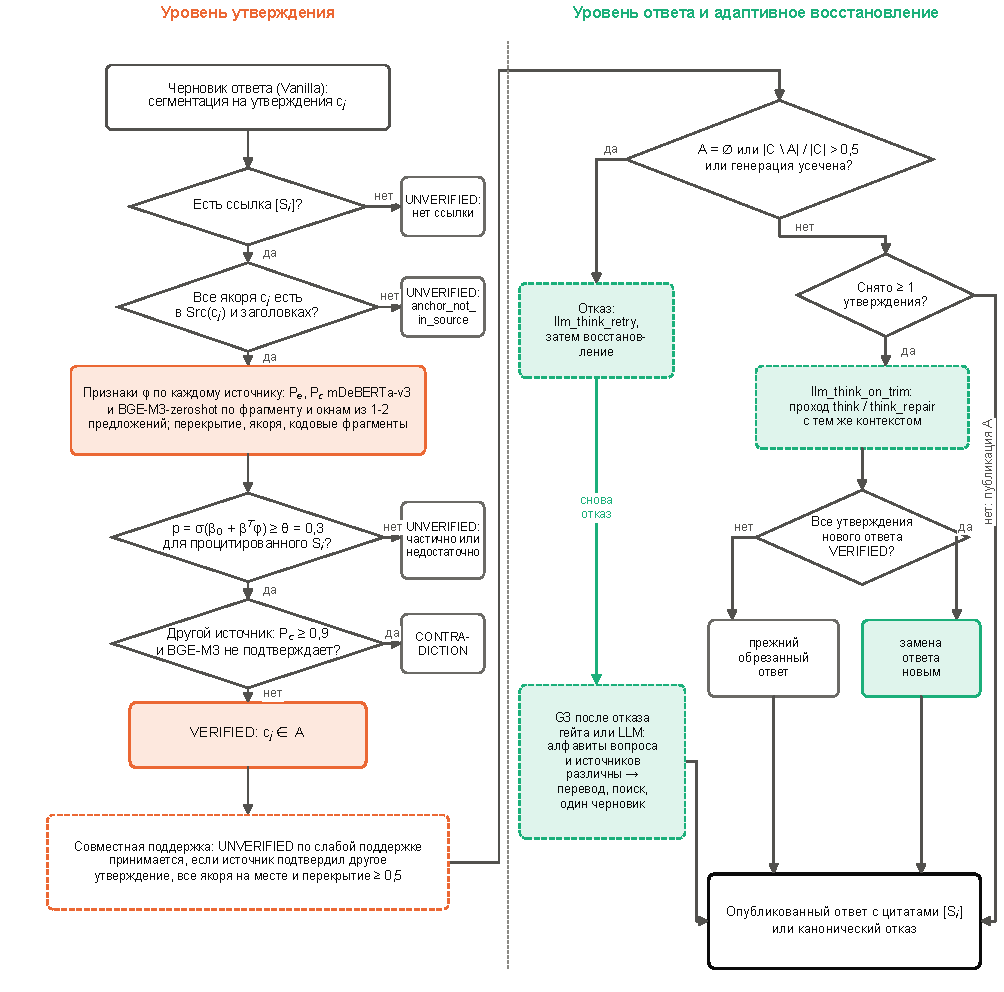
\includegraphics[width=\textwidth]{figures/fig3.pdf}
\caption{Рисунок 3 – Блок-схема политики допуска утверждений, проверки якорей и адаптивного восстановления}
\end{figure}

Сквозная диагностика реализована типизированным результатом RAGResponse. Для каждого запроса сохраняются времена стадий, оценки BM25, плотного поиска, RRF и кросс-энкодера для каждого кандидата, все попытки генерации и их проверка, вероятности обеих NLI-моделей с текстом фактической посылки, оценка судьи и причина отказа. Такая трассировка позволяет повторно проверить любой черновик новой версией верификатора без обращения к генератору.

\subsection*{\textit{Адаптивные механизмы восстановления полноты и преодоления отказов}}
Независимая проверка надёжно отсекает неподтверждённые утверждения, но в составных ответах снимает и верные утверждения с неуверенной оценкой, а генератор часто отказывается при межъязыковом расхождении вопроса и источника. Для этих случаев введены четыре прохода, каждый из которых запускается только по формальному условию.

Проход с рассуждением после отказа (llm\_think\_retry) повторяет генерацию с включённым рассуждением на том же контексте, если ответ отклонён по любой причине, кроме превышения бюджета контекста.

Проход с рассуждением после обрезки (llm\_think\_on\_trim) запускается, если опубликованный черновик без рассуждения содержит хотя бы одно снятое утверждение. Пусть $r_0$ – проверенный черновик, $r_1$ – проверенный ответ прохода с рассуждением (think и, при необходимости, think\_repair) на том же контексте. Публикуемый результат определяется правилом

\begin{equation}
r^{*} = \begin{cases} r_1, & \Phi(r_0, r_1), \\ r_0, & \neg\, \Phi(r_0, r_1), \end{cases}
\tag{9}
\end{equation}
\noindent где $\Phi(r_0, r_1) = \neg\, \mathrm{refuse}(r_0) \wedge C_0 \ne \mathcal{A}_0 \wedge \neg\, \mathrm{refuse}(r_1) \wedge C_1 = \mathcal{A}_1$ – условие замены: черновик опубликован, но обрезан, а новый ответ опубликован и проверен полностью; $C_0, \mathcal{A}_0$ и $C_1, \mathcal{A}_1$ – утверждения и допущенные утверждения черновика и нового ответа. Новый ответ заменяет исходный только при полной проверке всех его утверждений, поэтому по построению правило не может заменить опубликованный ответ менее проверенным.

Восстановление (llm\_recovery) после отказа самого генератора запрашивает две дополнительные выборки при температуре 0,7, если лучший фрагмент имеет оценку кросс-энкодера не ниже 0,5; публикуется первая выборка, прошедшая политику допуска.

Перевод вопроса после отказа (G3, QUERY\_TRANSLATION) направлен на межъязыковой разрыв. Пусть $\mathrm{scr}(x) \in \{\mathrm{ru}, \mathrm{en}\}$ – преобладающий алфавит текста по числу кириллических и латинских букв, $S$ – тексты источников, показанных генератору, или пяти лучших кандидатов переранжирования, если отказ дал гейт. Перевод запускается при условии

\begin{equation}
\mathrm{G3}(q) \iff \rho(q) \in \{\rho_{\mathrm{gate}},\, \rho_{\mathrm{LLM}}\} \;\wedge\; \mathrm{scr}(q) \ne \mathrm{scr}(S)
\tag{10}
\end{equation}
\noindent где $\rho(q)$ – причина отказа на вопрос $q$; $\rho_{\mathrm{gate}}$ – отказ гейта релевантности (relevance\_threshold\_not\_met); $\rho_{\mathrm{LLM}}$ – отказ генератора (llm\_refusal). Генератор одним вызовом без источников и без рассуждения переводит вопрос на язык источников, сохраняя имена, числа и идентификаторы; ответ длиннее $3|q| + 40$ символов отбрасывается как попытка ответить вместо перевода.

\subsection*{\textit{Экспериментальный стенд и методология оценки}}
Полные прогоны конвейера выполнены на вычислительном стенде под управлением Linux с видеокартой NVIDIA GeForce RTX 3090 (24 ГБ видеопамяти); использованы Python 3.12, PyTorch 2.11 с CUDA 12.8, transformers 5.12, sentence-transformers 5.2, qdrant-client 1.16 и rank-bm25 0.2.2. Офлайн-воспроизведение залогированных черновиков, анализ ошибок и проверка гипотез выполнены на ноутбуке с процессором Intel Core Ultra 7 255H, 48 ГБ оперативной памяти и видеокартой NVIDIA GeForce RTX 5060 Laptop (8 ГБ): повтор (offline.py, B00) заново проверяет все залогированные черновики текущим кодом верификатора с кэшированием предсказаний NLI, не обращаясь к генератору.

Оценочный набор включает 1307 вопросов (таблица 2). Технический набор v3 содержит 220 вопросов по девяти документам: RFC 9000 [27], RFC 9110 [28], RFC 9457 [29], RFC 9562 [30], NIST SP 800-53 Rev. 5 [31], NIST SP 800-63B-4 [32], документации PostgreSQL 18 [33] и PEP 703 [34]. Вопросы относятся к шести категориям: одношаговые, многошаговые, табличные и кодовые, лексические ловушки, состязательные (с ложной предпосылкой) и неотвечаемые; половина вопросов задана на русском языке к англоязычным документам. Набор XQuAD full построен на основе параллельного корпуса XQuAD [35; 36]: корпусом служат русскоязычные абзацы 40 статей, отвечаемые вопросы заданы на русском и на английском языке, а неотвечаемые относятся к восьми статьям, исключённым из корпуса.

\begin{table}[htbp]
\begin{singlespace}\footnotesize
\noindent Таблица 2 – Состав оценочного набора\\[2pt]
\begin{tabularx}{\textwidth}{YYYYYY}
\toprule
\textbf{Набор} & \textbf{Вопросов} & \textbf{Отвечаемые} & \textbf{Неотвечаемые и состязательные} & \textbf{Язык вопросов} & \textbf{Корпус} \\
\midrule
v3 & 220 & 127 & 93 (48 неотвечаемых, 45 состязательных) & 109 RU, 111 EN & 9 англоязычных стандартов и спецификаций \\
XQuAD full & 1087 & 911 & 176 & 552 RU, 535 EN & 40 русскоязычных статей \\
Всего & 1307 & 1038 & 269 & 661 RU, 646 EN & – \\
\bottomrule
\end{tabularx}
\end{singlespace}
\end{table}

Для каждого вопроса фиксируются три исхода. Ответ верен, если для отвечаемого вопроса опубликованный текст содержит все обязательные факты эталона, а для неотвечаемого и состязательного вопроса система отказала или явно опровергла ложную предпосылку. Галлюцинацией считается опубликованное фактическое утверждение в ответ на неотвечаемый или состязательный вопрос (269 вопросов), ложным отказом считается отказ на отвечаемый вопрос (1038 вопросов). Столбец Vanilla отражает черновик генератора до верификации, столбец FactRAG – опубликованный результат.

Разбиение на выборки dev (651 вопрос) и test (656 вопросов) выполнено один раз, стратифицировано по набору и категории, для XQuAD сгруппировано по абзацам и заморожено: все пороги и решения о включении механизмов принимались только по dev. Каждый прогон записывает хеши SHA-256 файлов кода, датасетов и моделей; загрузчики проверяют хеш датасета перед сравнением, а эталонные метки на протяжении всех итераций не изменялись. Конфигурации сравниваются попарно по вопросам точным двусторонним тестом Мак-Немара [37]:

\begin{equation}
p = \min\left(1,\; 2 \sum_{i=0}^{\min(b, c)} \binom{b + c}{i} \, 2^{-(b + c)}\right)
\tag{11}
\end{equation}
\noindent где $b$ – число вопросов, ставших верными; $c$ – число вопросов, ставших неверными; вопросы с одинаковым исходом в тест не входят.

Каждая гипотеза вводилась отдельным флагом, выключенным по умолчанию, и принималась при одновременном выполнении четырёх заранее заданных критериев: воспроизводимый прирост, отсутствие новых галлюцинаций, отсутствие потерь ранее верных ответов и прирост на выборке dev. Порядок проверки включал офлайн-повтор на ноутбуке, шаговый контур на RTX 3090 (steps.py), в котором выполняются только новые вызовы генератора от залогированного состояния, сквозной прогон затронутых вопросов с контрольной группой и полный прогон на 1307 вопросах.

\section*{Результаты}
\subsection*{\textit{Качество поиска и межъязыковой разрыв}}
В итоговой конфигурации на наборе XQuAD достигнуты Recall@5 = 0,981 и MRR@10 = 0,966; гейт релевантности отклоняет 81,8 \% неотвечаемых вопросов (144 из 176) и 1,4 \% отвечаемых (13 из 911). На техническом наборе v3 структурный разбор parser v2 повысил Recall@5 с 0,837 до 0,907 и MRR@10 с 0,769 до 0,824. Гейт на v3 не отклоняет неотвечаемые вопросы: они относятся к тем же документам (смежный раздел, ложная предпосылка, другая версия стандарта), и переранжировщик оценивает тематическую близость, а не наличие ответа; площадь под ROC-кривой лучшей оценки для разделения отвечаемых и неотвечаемых вопросов составляет 0,764 на v3 против 0,991 на XQuAD. Неотвечаемые вопросы v3 удерживает второй рубеж: отказ генератора и верификатор.

Межъязыковой разрыв проявляется в оценках переранжировщика (рисунок 4). Для 52 упорных отказов на XQuAD, то есть отвечаемых вопросов, на которые все попытки (черновик, рассуждение, восстановление) дали отказ, медианная оценка эталонного фрагмента составляет 0,089 на английском языке против 0,802 у остальных вопросов и 0,588 против 0,988 на русском. Эксперимент E3 с эталонным русским переводом английских вопросов из параллельного корпуса показал потенциал перевода: медиана лучшей оценки выросла с 0,781 до 0,976, гейт пропустил 445 отвечаемых вопросов из 447 вместо 437, а эталонный фрагмент оказался первым в 433 случаях вместо 418.

\begin{figure}[htbp]\centering
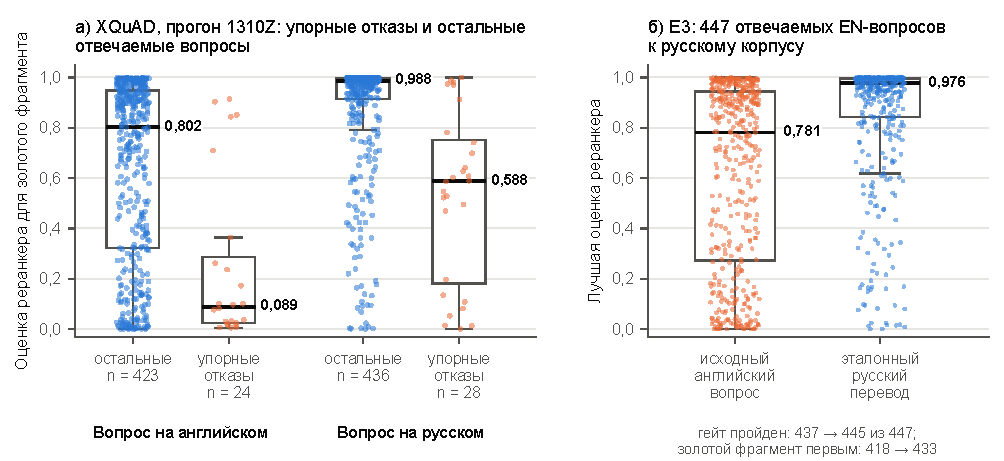
\includegraphics[width=\textwidth]{figures/fig4.pdf}
\caption{Рисунок 4 – Оценки переранжировщика: а) эталонный фрагмент для упорных отказов и остальных отвечаемых вопросов XQuAD (прогоны 1310Z и 1222Z дают одинаковые оценки); б) лучшая оценка до и после эталонного перевода английских вопросов (E3)}
\end{figure}

\subsection*{\textit{Сквозная точность по рубежам оптимизации}}
Динамика сквозной точности на 1307 вопросах представлена в таблице 3 и на рисунке 5а. Исходная конфигурация (прогон 0749Z) дала 90,2 \% верных ответов. Исправление нормализации якорей и правило llm\_think\_on\_trim (прогон 1310Z) повысили точность до 90,6 \% за счёт технического набора (с 86,4 до 88,6 \%, со 190 до 195 вопросов) при неизменных 91,0 \% на XQuAD; попарно +5/−0, $p = 0{,}0625$. Перевод вопроса G3 (прогон 1929Z) сократил ложные отказы с 79 до 74 и повысил точность до 90,9 \%: попарно +4/−0 по оценщику и +5/−0 фактически, по +2 вопроса на dev и на test, без новых галлюцинаций. Структурный разбор parser v2 (прогон 1222Z) повысил точность на v3 до 90,9 \% и общую до 91,3 \%; попарно +11/−6, $p = 0{,}33$, при этом все 1087 ответов XQuAD совпали с предыдущим прогоном дословно.

\begin{table}[htbp]
\begin{singlespace}\footnotesize
\noindent Таблица 3 – Сквозные метрики по рубежам оптимизации, \% (число вопросов)\\[2pt]
\begin{tabularx}{\textwidth}{YYYYY}
\toprule
\textbf{Метрика} & \textbf{0749Z исходная} & \textbf{1310Z якоря, think\_on\_trim} & \textbf{1929Z + G3} & \textbf{1222Z + parser v2} \\
\midrule
Верно, все 1307 & 90,2 (1179) & 90,6 (1184) & 90,9 (1188) & 91,3 (1193) \\
Верно, v3 (220) & 86,4 (190) & 88,6 (195) & 88,6 (195) & 90,9 (200) \\
Верно, XQuAD (1087) & 91,0 (989) & 91,0 (989) & 91,4 (993) & 91,4 (993) \\
Черновик Vanilla, все & 86,0 (1124) & 86,0 (1124) & 86,1 (1125) & 86,7 (1133) \\
Галлюцинации (из 269) & 1,1 (3) & 1,1 (3) & 1,1 (3) & 0,7 (2) \\
Ложные отказы (из 1038) & 7,6 (79) & 7,6 (79) & 7,1 (74) & 6,7 (70) \\
Попарно к предыдущему & – & +5/−0, p = 0,0625 & +4/−0, p = 0,125 & +11/−6, p = 0,33 \\
\bottomrule
\end{tabularx}
\end{singlespace}
\end{table}

Отдельные шаги, взятые по одному, не достигают статистической значимости. Суммарный эффект всей оптимизации, то есть сравнение итогового прогона 1222Z с исходным 0749Z по каждому вопросу, составил +18/−4 при $p = 0{,}0043$, причём прирост распределён поровну между выборками: +9/−2 на dev и +9/−2 на test. Из четырёх потерь две вызваны оценщиком (V3-MH-028, V3-UNA-028), две связаны с проверкой таблиц (V3-TC-022, V3-TC-025). Верификатор повышает долю верных ответов над черновиком генератора с 86,7 до 91,3 \%.

Для сравнения с ранним прототипом использован тот же набор v3. Прототип (Qwen2.5-14B-Instruct, верификатор первой версии, RTX 5060 Laptop) дал 75,5 \% верных ответов при 4,3 \% галлюцинаций и 18,9 \% ложных отказов и медианном времени ответа 21,4 с; итоговая конфигурация на том же наборе даёт 90,9 \% верных ответов, 2,2 \% галлюцинаций (2 из 93) и 2,4 \% ложных отказов (3 из 127) при медианном времени 6,1 с. Сравнение отражает совокупный эффект смены генератора, переранжировщика, верификатора и оборудования и не является абляцией отдельных компонентов.

\begin{figure}[htbp]\centering
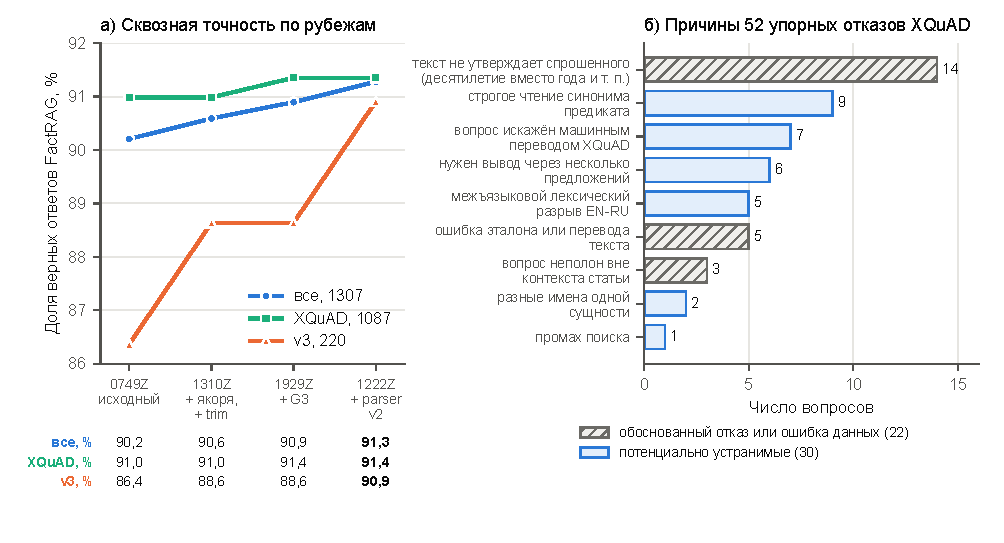
\includegraphics[width=\textwidth]{figures/fig5.pdf}
\caption{Рисунок 5 – Эволюция сквозной точности и структура упорных отказов: а) доля верных ответов по рубежам оптимизации; б) причины 52 упорных отказов на XQuAD (прогон 1310Z)}
\end{figure}

\subsection*{\textit{Распределение оценок верификатора}}
На рисунке 6 показаны все 1357 фактических утверждений, проверенных в итоговом прогоне 1222Z во всех попытках генерации. Допущены 1252 утверждения; 74 сняты по низкой оценке судьи, 13 – по противоречию, 18 – фильтром якорей. Облако допущенных утверждений сосредоточено в области высокой вероятности следования обеих моделей, тогда как снятые утверждения распределены по всей плоскости: классификаторы часто расходятся, и судья учитывает обе оценки вместе с признаками якорей. Фильтр якорей снимает утверждения независимо от оценки судьи: утверждение V3-TC-022 о поле node идентификатора UUIDv1 получило оценку 0,993, но идентификатор находился в соседнем фрагменте документа и в процитированном источнике отсутствовал. В промежуточном прогоне 1310Z тем же механизмом было снято утверждение V3-MH-024 об усилении AC-7(4) с оценкой 0,643; в итоговом прогоне структурный разбор связал метку усиления с её текстом, и ответ стал верным. Отмеченные на рисунке случаи V3-MH-002, V3-TC-021 и V3-TC-025 разобраны в разделе «Обсуждение».

\begin{figure}[htbp]\centering
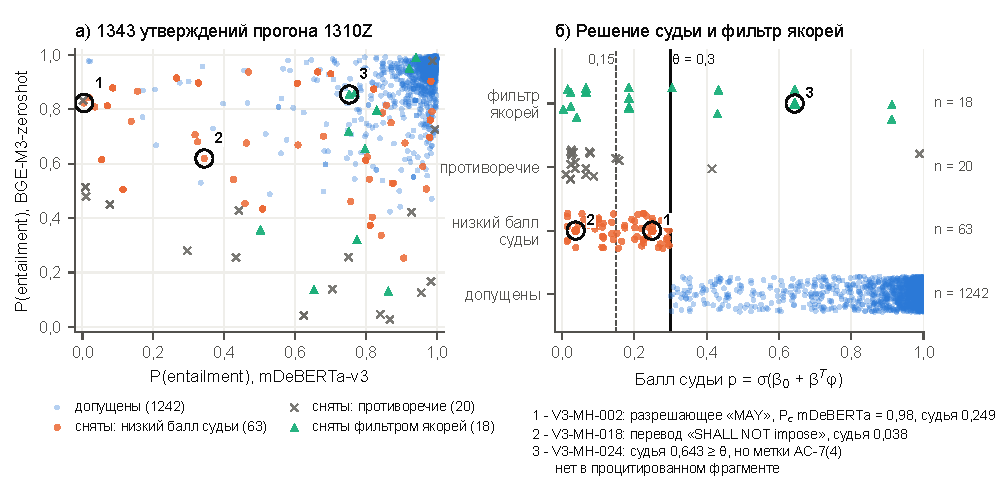
\includegraphics[width=\textwidth]{figures/fig6.pdf}
\caption{Рисунок 6 – Оценки верификатора для 1357 утверждений итогового прогона 1222Z: а) вероятности следования mDeBERTa-v3 и BGE-M3-zeroshot; б) оценка судьи по исходам проверки}
\end{figure}

\subsection*{\textit{Воспроизводимость}}
Контур детерминирован на всех уровнях проверки. Между прогонами 0749Z и 1310Z дословно совпали 1300 итоговых ответов из 1307 (из 1005 ответов, опубликованных в обоих прогонах, совпали 998); между 1310Z и 1929Z совпали 1302 ответа. Офлайн-повтор B00 залогированных черновиков текущим кодом воспроизводит 1307 исходов из 1307. Контроль D0 шагового контура на RTX 3090 воспроизвёл 6 из 6 первых черновиков. Сквозной прогон G3 (1839Z) на 151 вопросе популяции и 20 контрольных вопросах дал те же 151 перевод, те же пять опубликованных ответов дословно и тот же попарный результат, что и шаговый контур; контрольные вопросы не изменились. Полный прогон 1929Z дал ровно спрогнозированные 1188 верных ответов.

\subsection*{\textit{Проверка гипотез}}
Результаты проверки гипотез сведены в таблицу 4. В рабочую конфигурацию вошли только изменения, выполнившие все четыре критерия; изменения с приростом только на test оставлены кандидатами за выключенными флагами.

\begin{table}[htbp]
\begin{singlespace}\footnotesize
\noindent Таблица 4 – Проверенные гипотезы и абляционные эксперименты\\[2pt]
\begin{tabularx}{\textwidth}{YYYY}
\toprule
\textbf{Гипотеза} & \textbf{Суть изменения} & \textbf{Результат} & \textbf{Решение} \\
\midrule
X00 & исправление нормализации разделителей в якорях & +1/−0 (V3-MH-001), устранена ошибка кода & принято \\
llm\_think\_on\_trim & рассуждение после обрезки, замена только при полной проверке & 16 срабатываний: 4 исправления, 0 ухудшений, 0 новых галлюцинаций & принято \\
Порог судьи & $\theta$ от 0,20 до 0,35 на dev & 0,2: +1 верный ответ при росте принятия ложных утверждений & $\theta = 0{,}3$ подтверждён \\
Маршрутизатор рассуждения & пропуск рассуждения при низкой оценке переранжировщика & на dev теряется от 1 до 15 верных ответов & отвергнуто \\
E1 & идентификатор из соседнего фрагмента того же документа & +1/−0 только на test (V3-MH-024); полных составных ответов 69 → 70 из 84 & кандидат \\
E2 & развёртывание одностолбцовых таблиц в текст & 0 изменений; причина в NLI на модальности & отвергнуто \\
E3 & эталонный перевод вопроса (оракул) & гейт 437 → 445 из 447; медиана 0,781 → 0,976 & потенциал подтверждён \\
E4 & поиск по частям составного вопроса & фрагменты доказательства 29 → 30 из 39; 0 на неверных & отвергнуто \\
E5, G2 & добавление соседнего фрагмента & E5: дорого без триггера; G2: +1 только на test & кандидат \\
G3 & перевод вопроса после отказа & +4/−0 (+5 фактически), dev +2, test +2; 0 из 119 неотвечаемых опубликовано & принято \\
G4 & нормализация вопроса после отказа LLM & 140 вопросов: 85 без изменений, 55 снова отказ; +0/−0 & отвергнуто \\
parser v2 & структурный разбор таблиц и заголовков & v3: 195 → 200; +11/−6, 0 изменений на XQuAD & принято \\
T1 & окно NLI на каждую строку таблицы & +1 только на test; рост принятия ложных табличных утверждений & отвергнуто \\
\bottomrule
\end{tabularx}
\end{singlespace}
\end{table}

Правило llm\_think\_on\_trim в живом прогоне сработало на 16 вопросах: четыре ответа исправлено, семь уже были верны (в трёх из них ответ заменён более полным проверенным), пять остались неверными, и ни один ответ не ухудшился. Для гипотезы G3 популяция составила 151 вопрос (90 отказов гейта и 61 отказ генератора). После перевода опубликовано пять ответов, все на английские вопросы к русскому корпусу; один из них (V3-XQFEN-320) верен, но не засчитан оценщиком. Из 113 неотвечаемых вопросов популяции после перевода 42 прошли гейт, однако ни один не был опубликован. Гипотеза E1 безопасна и воспроизводима на двух прогонах, но её единственный прирост приходится на test, поэтому она оставлена кандидатом. Гипотеза G4 опровергнута: модель почти не меняет формулировку, а изменённые вопросы снова получают отказ, то есть формулировка вопроса не является причиной отказов.

\subsection*{\textit{Время отклика и стоимость адаптивных контуров}}
В итоговом прогоне медианное время генерации на RTX 3090 составило 5,5 с на наборе v3 и 4,0 с на XQuAD, полного ответа – 6,1 и 4,4 с соответственно (рисунок 7а); в прогоне 1310Z до введения нового разбора эти значения составляли 5,6 и 6,4 с на v3. Генерация занимает от 89 до 91 \% времени ответа; гибридный поиск, переранжирование и проверка двумя NLI-моделями вместе занимают менее 0,5 с. Пиковое потребление видеопамяти по снимкам журнала прогона 0749Z составило 21,9 ГБ из 24 ГБ.

Условные контуры увеличивают время только на сработавших вопросах (рисунок 7б). Стоимость перевода G3 измерена попарно: те же 151 вопрос в сквозном прогоне 1839Z с переводом и в прогоне 1310Z без него. Перевод добавляет в медиане 4,1 с на переведённый вопрос (в среднем 2,9 с, максимум 8,4 с), из которых сам вызов перевода занимает около 0,6 с: распределение двухмодально, поскольку 75 переведённых вопросов из 151 не проходят гейт и не требуют генерации, а остальные получают новый черновик. На 151 вопрос популяции это 7,2 минуты на полный прогон. В итоговом прогоне перевод сработал также на 151 вопросе и опубликовал семь ответов. Проход llm\_think\_on\_trim в итоговом прогоне сработал на 13 вопросах и стоит в медиане 20,6 с на вопрос (в среднем 23,6 с), что добавляет около 5,1 минуты на прогон. Полный прогон 1307 вопросов занимает около трёх часов.

\begin{figure}[htbp]\centering
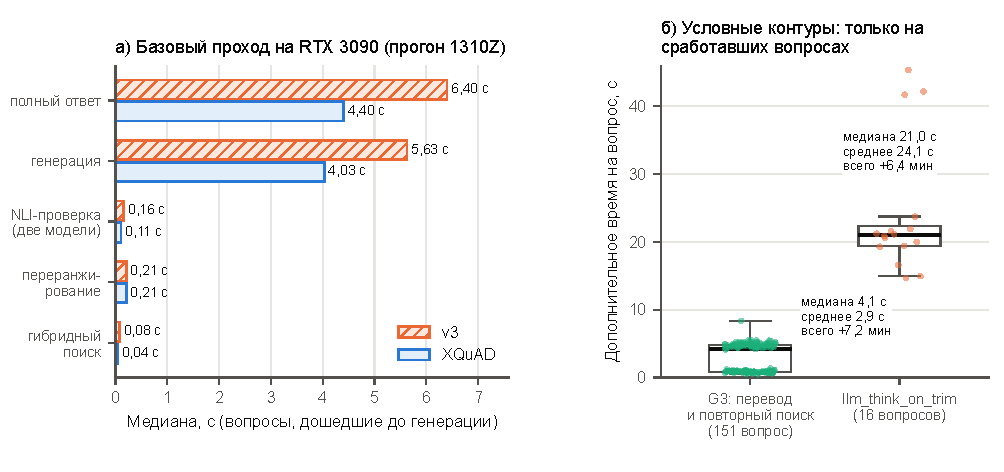
\includegraphics[width=\textwidth]{figures/fig7.pdf}
\caption{Рисунок 7 – Время отклика на RTX 3090: а) медианное время стадий в итоговом прогоне 1222Z; б) дополнительное время условных контуров на сработавших вопросах}
\end{figure}

\section*{Обсуждение}
Полученные результаты позволяют сделать четыре вывода. Первый касается структуры остаточных ошибок. Из 52 упорных отказов на XQuAD 22 представляют собой методологически обоснованные отказы или ошибки данных (рисунок 5б). В 14 случаях текст не утверждает того, о чём спрашивает вопрос: вопрос требует года, а текст называет десятилетие; вопрос спрашивает место рождения, а текст называет страну деятельности; вопрос спрашивает численность, а текст приводит долю. Отказ в этих случаях соответствует назначению контура, хотя оценщик засчитывает его как ошибку. В пяти случаях эталон или перевод текста XQuAD противоречит вопросу; так, в V3-XQFEN-245 английское «jawless» (бесчелюстные) переведено в тексте корпуса как «челюстноротые». Ещё три вопроса неполны вне контекста статьи («этот лидер», «университет»). Реалистичный резерв составляют 12 вопросов с искажённым переводом и межъязыковым лексическим разрывом и часть из девяти вопросов со строгим чтением синонима предиката. Перевод G3 не устранил ни одного случая лексического разрыва: перевод генератора не попадает в термин текста («Nationality Act» против «Закона о гражданстве»), что указывает на потребность в словаре терминов, а не в переформулировании.

Второй вывод касается безопасности адаптивных контуров. После перевода 42 неотвечаемых вопроса прошли гейт релевантности, то есть первый рубеж перестал их удерживать, но ни один не был опубликован: их удержал отказ генератора, и верификатору не потребовалось снимать утверждения. В сквозном прогоне на 119 неотвечаемых вопросах не опубликован ни один ответ. Вместе с тем безопасность этой группы держится на одном рубеже, и при смене генератора её необходимо проверять заново.

Третий вывод касается фундаментальных ограничений NLI-верификации. Классификатор mDeBERTa-v3 присваивает вероятность противоречия 0,98 верному утверждению «по коду 302 агент может сменить метод с POST на GET» (V3-MH-002): разрешающая модальность MAY в источнике и тот факт, что субъект «302 Found» находится только в заголовке раздела, приводят к оценке судьи 0,249 ниже порога. В V3-MH-018 перевод требования «SHALL NOT impose other composition rules» получил оценку 0,038, а ответ прохода с рассуждением смешал русский и английский языки, и все его утверждения были сняты как противоречащие; в итоговом прогоне ответ на этот вопрос верен, но сама чувствительность NLI к смешению языков сохраняется. В V3-MH-036 значение PYTHONGIL=1 оказалось отрезано границей фрагмента, и утверждение не могло пройти контроль якорей. Табличные вопросы образуют отдельный класс: при подаче всей таблицы как одной посылки классификатор не связывает значение со своей строкой (V3-TC-021), а битовый шаблон, разнесённый по ячейкам «1 | 0 | 0 | 0», не совпадает с якорем «1000» (V3-TC-025). В V3-TC-022 судья подтверждает утверждение с оценкой 0,993, но идентификатор находится в соседнем фрагменте того же документа; именно такие случаи устраняет кандидат E1, который в повторе итогового прогона даёт +1 ответ на выборке test. Экспериментальная проверка окон NLI по строкам таблицы (T1) показала, что такие окна повышают принятие верных табличных утверждений, но повышают и принятие ложных: на стресс-наборе из 784 шаблонных утверждений по 27 таблицам ложное утверждение со значением соседней строки принимается в 66 \% случаев на английском и 89 \% на русском уже в текущей конфигурации и в 72 и 93 \% с окнами строк. Вероятностная проверка таблиц, таким образом, требует дополнения детерминированным правилом привязки ключа и значения к одной строке.

Единственная истинная числовая галлюцинация промежуточных прогонов V3-ADV-029 возникла по сходному механизму: на вопрос «содержит ли поле rand\_b 74 бита» модель трижды написала верную поправку «поле rand\_b содержит 62 бита», но поправка снималась, поскольку якорь UUIDv7 отсутствовал в процитированном фрагменте, а следующее, дословно верное утверждение о 74 битах полей rand\_a и rand\_b публиковалось и подтверждало ложную предпосылку. В прогоне 1222Z новый структурный разбор дал генератору иной контекст, верная поправка прошла проверку и была опубликована; этот случай показывает, почему ответ, начинающийся с опровержения предпосылки, отклоняется при снятии обосновывающего утверждения. Две галлюцинации итогового прогона не являются выдуманными фактами: в V3-ADV-013 верный ответ «не менее чем в три раза» не распознан шаблоном оценщика, а в V3-UNA-028 на неотвечаемый вопрос опубликована дословно подтверждённая фраза источника о поддерживаемых методах сжатия.

Четвёртый вывод касается автоматического оценщика. Шаблоны засчитывают ошибкой часть верных ответов: в эталоне V3-XQFEN-320 слово «бoльшим» записано с латинской буквой «o», и правило не находит кириллическое написание в дословно совпадающем ответе; шаблон V3-MH-028 не принимает слово «ноль»; шаблон V3-ADV-013 не содержит формы «три». Эталоны сознательно не исправлялись задним числом: изменение меток между итерациями сделало бы попарные сравнения несопоставимыми и открыло бы возможность подгонки оценки под результат. Исправленные шаблоны должны вводиться как новая версия разметки с отдельной строкой в отчётах.

В сравнении с модульными каркасами LangChain, LlamaIndex и Haystack [38; 39; 40] контур отличается не набором компонентов, а фиксированными обязательствами: политика допуска закреплена в конвейере, отказ является штатным исходом, адаптивные проходы не могут опубликовать непроверенный текст, а диагностика каждого решения сохраняется без дополнительной инструментальной обвязки (таблица 5).

\begin{table}[htbp]
\begin{singlespace}\footnotesize
\noindent Таблица 5 – Сопоставление с модульными каркасами\\[2pt]
\begin{tabularx}{\textwidth}{YYYYY}
\toprule
\textbf{Критерий} & \textbf{LangChain} & \textbf{LlamaIndex} & \textbf{Haystack} & \textbf{FactRAG-NLI} \\
\midrule
Конвейер & модульный & модульный & компонентный & фиксированный профиль \\
Цитирование & настраивается & специализированный модуль & настраивается & [S$_i$] и проверка каждого утверждения \\
Верификация & через маршруты & интегрируемая & циклы и ветвления & двухмодельный судья и контроль якорей \\
Восстановление & вручную & вручную & вручную & условные проходы с полной проверкой \\
Диагностика & зависит от сборки & источники & данные конвейера & оценки, вероятности NLI, балл судьи, причины отказа \\
\bottomrule
\end{tabularx}
\end{singlespace}
\end{table}

Ограничения исследования связаны с данными и стендом. Эталонная разметка набора v3 подготовлена с использованием языковой модели и не прошла независимую экспертную проверку; набор XQuAD содержит ошибки машинного перевода. Отдельные шаги оптимизации статистически незначимы, значим только их совокупный эффект, причём этот вывод опирается на одну последовательность прогонов. Все полные прогоны выполнены на одном аппаратном стенде с одним генератором; безопасность при смене генератора требует повторной проверки. Декомпозиция на уровне предложений не является полноценной семантической атомизацией, а распознавание текста отсканированных документов не реализовано.

\section*{Заключение}
В работе построен и экспериментально исследован локальный многорубежный контур FactRAG-NLI, в котором каждое утверждение ответа проходит независимую проверку. Все задачи исследования решены: реализована инкрементальная индексация со структурным разбором заголовков и таблиц; построен двухэтапный гибридный поиск BM25 и BGE-M3 с объединением Reciprocal Rank Fusion, весом по покрытию словаря, переранжированием bge-reranker-v2-m3 и гейтом релевантности; формализована двухмодельная верификация с логистическим судьёй и детерминированным контролем якорей; разработаны адаптивные механизмы llm\_think\_on\_trim и G3, публикующие только полностью проверенный текст; построена воспроизводимая методика оценки с замороженным разбиением dev/test, контролем хешей и точным тестом Мак-Немара.

На 1307 вопросах итоговая конфигурация даёт 91,3 \% верных ответов против 90,2 \% исходной (+18/−4, $p = 0{,}0043$, прирост поровну на dev и test), 90,9 \% на техническом наборе, 0,7 \% галлюцинаций и 6,7 \% ложных отказов при медианном времени полного ответа от 4,4 до 6,1 с на одной видеокарте. Проверка двумя NLI-моделями занимает от 0,1 до 0,2 с на ответ, тогда как на генерацию приходится от 89 до 91 \% времени. Дальнейшее развитие предполагает детерминированную привязку ключа и значения к строке таблицы, адаптацию NLI-модели к модальным конструкциям и отрицаниям на выборке dev, словарь межъязыковых терминов и псевдонимов сущностей, версионированную экспертную ревизию эталонной разметки и проверку контура с другими генераторами.

\section*{Список источников}
\begin{singlespace}\small
\begin{enumerate}
\item Ji Z., Lee N., Frieske R. [et al.]. Survey of Hallucination in Natural Language Generation // ACM Computing Surveys. 2023. Vol. 55, no. 12. Art. 248. P. 1–38. DOI: 10.1145/3571730.
\item Huang L., Yu W., Ma W. [et al.]. A Survey on Hallucination in Large Language Models: Principles, Taxonomy, Challenges, and Open Questions // ACM Transactions on Information Systems. 2025. Vol. 43, no. 2. Art. 42. P. 1–55. DOI: 10.1145/3703155.
\item Bradner S. Key words for use in RFCs to Indicate Requirement Levels : RFC 2119. IETF, 1997. DOI: 10.17487/RFC2119. URL: https://www.rfc-editor.org/rfc/rfc2119 (дата обращения: 05.11.2026).
\item Lewis P., Perez E., Piktus A. [et al.]. Retrieval-Augmented Generation for Knowledge-Intensive NLP Tasks // Advances in Neural Information Processing Systems. 2020. Vol. 33. P. 9459–9474.
\item Gao Y., Xiong Y., Gao X. [et al.]. Retrieval-Augmented Generation for Large Language Models: A Survey. 2023. arXiv:2312.10997. DOI: 10.48550/arXiv.2312.10997.
\item Gao T., Yen H., Yu J., Chen D. Enabling Large Language Models to Generate Text with Citations // Proceedings of the 2023 Conference on Empirical Methods in Natural Language Processing. 2023. P. 6465–6488. DOI: 10.18653/v1/2023.emnlp-main.398.
\item О коммерческой тайне : Федеральный закон от 29.07.2004 № 98-ФЗ (ред. действ.). Доступ из справ.-правовой системы «КонсультантПлюс».
\item Asai A., Wu Z., Wang Y., Sil A., Hajishirzi H. Self-RAG: Learning to Retrieve, Generate, and Critique through Self-Reflection // International Conference on Learning Representations (ICLR). 2024.
\item Min S., Krishna K., Lyu X. [et al.]. FActScore: Fine-grained Atomic Evaluation of Factual Precision in Long Form Text Generation // Proceedings of the 2023 Conference on Empirical Methods in Natural Language Processing. 2023. P. 12076–12100. DOI: 10.18653/v1/2023.emnlp-main.741.
\item Es S., James J., Espinosa-Anke L., Schockaert S. RAGAS: Automated Evaluation of Retrieval Augmented Generation // Proceedings of the 18th Conference of the European Chapter of the Association for Computational Linguistics: System Demonstrations. 2024. P. 150–158. DOI: 10.18653/v1/2024.eacl-demo.16.
\item Honovich O., Aharoni R., Herzig J. [et al.]. TRUE: Re-evaluating Factual Consistency Evaluation // Proceedings of the 2022 Conference of the North American Chapter of the Association for Computational Linguistics. 2022. P. 3905–3920. DOI: 10.18653/v1/2022.naacl-main.287.
\item Laban P., Schnabel T., Bennett P. N., Hearst M. A. SummaC: Re-Visiting NLI-based Models for Inconsistency Detection in Summarization // Transactions of the Association for Computational Linguistics. 2022. Vol. 10. P. 163–177. DOI: 10.1162/tacl\_a\_00453.
\item Robertson S., Zaragoza H. The Probabilistic Relevance Framework: BM25 and Beyond // Foundations and Trends in Information Retrieval. 2009. Vol. 3, no. 4. P. 333–389. DOI: 10.1561/1500000019.
\item Chen J., Xiao S., Zhang P. [et al.]. M3-Embedding: Multi-Linguality, Multi-Functionality, Multi-Granularity Text Embeddings Through Self-Knowledge Distillation // Findings of the Association for Computational Linguistics: ACL 2024. 2024. P. 2318–2335. DOI: 10.18653/v1/2024.findings-acl.137.
\item Qdrant : векторная база данных : [программное обеспечение]. URL: https://github.com/qdrant/qdrant (дата обращения: 05.11.2026).
\item Cormack G. V., Clarke C. L. A., Büttcher S. Reciprocal Rank Fusion Outperforms Condorcet and Individual Rank Learning Methods // Proceedings of the 32nd International ACM SIGIR Conference on Research and Development in Information Retrieval. 2009. P. 758–759. DOI: 10.1145/1571941.1572114.
\item Nogueira R., Cho K. Passage Re-ranking with BERT. 2019. arXiv:1901.04085. DOI: 10.48550/arXiv.1901.04085.
\item Xiao S., Liu Z., Zhang P. [et al.]. C-Pack: Packaged Resources to Advance General Chinese Embedding // Proceedings of the 47th International ACM SIGIR Conference on Research and Development in Information Retrieval. 2024. P. 641–649. DOI: 10.1145/3626772.3657878.
\item Li C., Liu Z., Xiao S., Shao Y. Making Large Language Models A Better Foundation For Dense Retrieval. 2023. arXiv:2312.15503. DOI: 10.48550/arXiv.2312.15503.
\item Yang A., Li A., Yang B. [et al.]. Qwen3 Technical Report. 2025. arXiv:2505.09388. DOI: 10.48550/arXiv.2505.09388.
\item Qwen3.8-27B : карточка модели : [электронный ресурс]. URL: https://huggingface.co/Qwen/Qwen3.8-27B (дата обращения: 05.11.2026).
\item Frantar E., Ashkboos S., Hoefler T., Alistarh D. GPTQ: Accurate Post-Training Quantization for Generative Pre-trained Transformers // International Conference on Learning Representations (ICLR). 2023.
\item llama.cpp : инференс больших языковых моделей на C/C++ : [программное обеспечение]. URL: https://github.com/ggml-org/llama.cpp (дата обращения: 05.11.2026).
\item He P., Gao J., Chen W. DeBERTaV3: Improving DeBERTa using ELECTRA-Style Pre-Training with Gradient-Disentangled Embedding Sharing // International Conference on Learning Representations (ICLR). 2023.
\item Laurer M., van Atteveldt W., Casas A., Welbers K. Less Annotating, More Classifying: Addressing the Data Scarcity Issue of Supervised Machine Learning with Deep Transfer Learning and BERT-NLI // Political Analysis. 2024. Vol. 32, no. 1. P. 84–100. DOI: 10.1017/pan.2023.20.
\item Laurer M., van Atteveldt W., Casas A., Welbers K. Building Efficient Universal Classifiers with Natural Language Inference. 2023. arXiv:2312.17543. DOI: 10.48550/arXiv.2312.17543.
\item Iyengar J., Thomson M. QUIC: A UDP-Based Multiplexed and Secure Transport : RFC 9000. IETF, 2021. DOI: 10.17487/RFC9000. URL: https://www.rfc-editor.org/rfc/rfc9000 (дата обращения: 05.11.2026).
\item Fielding R., Nottingham M., Reschke J. HTTP Semantics : RFC 9110. IETF, 2022. DOI: 10.17487/RFC9110. URL: https://www.rfc-editor.org/rfc/rfc9110 (дата обращения: 05.11.2026).
\item Nottingham M., Wilde E., Dalal S. Problem Details for HTTP APIs : RFC 9457. IETF, 2023. DOI: 10.17487/RFC9457. URL: https://www.rfc-editor.org/rfc/rfc9457 (дата обращения: 05.11.2026).
\item Davis K., Peabody B., Leach P. Universally Unique IDentifiers (UUIDs) : RFC 9562. IETF, 2024. DOI: 10.17487/RFC9562. URL: https://www.rfc-editor.org/rfc/rfc9562 (дата обращения: 05.11.2026).
\item Joint Task Force. Security and Privacy Controls for Information Systems and Organizations : NIST Special Publication 800-53, Revision 5. Gaithersburg : National Institute of Standards and Technology, 2020. DOI: 10.6028/NIST.SP.800-53r5.
\item Temoshok D., Galluzzo R., LaSalle C. [et al.]. Digital Identity Guidelines: Authentication and Authenticator Management : NIST Special Publication 800-63B-4. Gaithersburg : National Institute of Standards and Technology, 2025. DOI: 10.6028/NIST.SP.800-63B-4.
\item PostgreSQL 18 Documentation : CREATE TABLE ; Chapter 11. Indexes. The PostgreSQL Global Development Group, 2025. URL: https://www.postgresql.org/docs/18/ (дата обращения: 05.11.2026).
\item Gross S. PEP 703 – Making the Global Interpreter Lock Optional in CPython. Python Software Foundation, 2023. URL: https://peps.python.org/pep-0703/ (дата обращения: 05.11.2026).
\item Artetxe M., Ruder S., Yogatama D. On the Cross-lingual Transferability of Monolingual Representations // Proceedings of the 58th Annual Meeting of the Association for Computational Linguistics. 2020. P. 4623–4637. DOI: 10.18653/v1/2020.acl-main.421.
\item Rajpurkar P., Zhang J., Lopyrev K., Liang P. SQuAD: 100,000+ Questions for Machine Comprehension of Text // Proceedings of the 2016 Conference on Empirical Methods in Natural Language Processing. 2016. P. 2383–2392. DOI: 10.18653/v1/D16-1264.
\item McNemar Q. Note on the Sampling Error of the Difference Between Correlated Proportions or Percentages // Psychometrika. 1947. Vol. 12, no. 2. P. 153–157. DOI: 10.1007/BF02295996.
\item LangChain : [программное обеспечение]. URL: https://github.com/langchain-ai/langchain (дата обращения: 05.11.2026).
\item LlamaIndex : [программное обеспечение]. URL: https://github.com/run-llama/llama\_index (дата обращения: 05.11.2026).
\item Haystack : [программное обеспечение]. URL: https://github.com/deepset-ai/haystack (дата обращения: 05.11.2026).
\end{enumerate}
\end{singlespace}
\begin{singlespace}\small
\textbf{Информация об авторе}

Е. Д. Мясников – студент факультета искусственного интеллекта Российского университета дружбы народов имени Патриса Лумумбы.

\textbf{Information about the author}

E. D. Myasnikov – Student, Faculty of Artificial Intelligence, Peoples' Friendship University of Russia named after Patrice Lumumba.

\end{singlespace}
\end{document}
